В этой главе обсуждаются эксперименты.

\section{Эксперимент на англоязычном наборе данных}
Для выбора оптимальной архитектуры основной системы был проведён пилотный эксперимент на открытых англоязычных данных. Цель эксперимента -- установить базовые показатели качества, выявить типичные ошибки парсинга на каждом этапе конвейера и обосновать необходимость гибридного подхода. В качестве эталонной разметки использовались файлы в форматах JATS/NLM XML, предоставляемые издателями вместе с PDF-версиями статей. Эти данные содержат аннотированные библиографические списки, что позволяет проводить автоматическое сравнение без ручной разметки.

Эксперименты проводились на четырёх подвыборках из официального репозитория \textit{GROBID end-to-end benchmarking datasets}:
\begin{itemize}
    \item \textbf{PMC\_sample\_1943}: 1\,943 статьи из PubMed Central (объём 1,5~Гб). Содержат PDF и NLM XML с метаданными и библиографией.
    \item \textbf{biorxiv-10k-test-2000}: 2\,000 препринтов bioRxiv (5,4~Гб). Включают PDF, аннотированные NLM XML, данные о финансировании и ссылках.
    \item \textbf{PLOS\_1000}: 1\,000 статей издательства PLOS (1,3~Гб). Полная структурная разметка в формате JATS XML.
    \item \textbf{eLife\_984}: 984 статьи eLife (4,5~Гб). PDF, JATS XML и HTML-версии.
\end{itemize}
Корпус охватывает различные издательские стили, двухколоночную и одноколоночную вёрстку, а также документы разной степени зашумлённости (наличные сканы, нестандартные шрифты, вложенные таблицы в разделах литературы).

Сравнение проводилось для трёх подходов:
\begin{enumerate}
    \item Гибридный метод сегментации текста~\cite{kopanichuk2025structure}. Комбинация эвристических правил, анализа макета страницы и регулярных выражений для поиска заголовков раздела библиографии и последующего чанкинга записей.
    \item GROBID. Запуск через REST API с последующим парсингом TEI/XML-ответа. Модель использует CRF-ансамбль, обученный на миллионах англоязычных статей.
    \item Пилотное тестирование LLM (Qwen2.5). Первоначально использовалась модель \texttt{Qwen2.5-32B-Instruct}. Из-за ограничений видеопамяти и экспоненциального роста потребления VRAM механизмом внимания при длинных контекстах модель была заменена на \texttt{Qwen2.5-14B-Instruct} с 4-битным квантованием (GGUF/AWQ). Обработка выполнялась постранично с выделением блока библиографии.
\end{enumerate}

Все эксперименты проводились на сервере с GPU NVIDIA Tesla V100-SXM2 (32~Гб VRAM), 64~Гб ОЗУ и процессоре Intel Xeon Gold. Для LLM применялся фреймворк \texttt{vLLM} с параметром \texttt{max\_model\_len=8192} и \texttt{gpu\_memory\_utilization=0.9}.

Качество оценивалось на трёх уровнях:
\begin{enumerate}
    \item Детекция границы библиографии: совпадение предсказанного и эталонного начала раздела (допуск $\pm$1 строка).
    \item Извлечение библиографических записей: посимвольное совпадение блоков с учётом нормализации пробелов и переносов.
    \item Извлечение авторов: точное совпадение последовательности имён/инициалов/фамилий в каждой записи.
\end{enumerate}
В качестве метрик использовались Precision и макро-$F_1$-мера. Оценка реализована через кастомный скрипт, сопоставляющий предсказанные и эталонные токены с учётом порядка и нормализации пунктуации.

\begin{table}[h]\centering
\footnotesize
\setlength{\tabcolsep}{3pt}
\renewcommand{\arraystretch}{1.2}
\caption{Результаты сравнения методов на англоязычном корпусе}
\label{tab:eng_benchmark}
\begin{tabularx}{\textwidth}{@{} l *{4}{>{\centering\arraybackslash}X} @{}}
\hline
\multirow{2}{*}{Метод} & \multicolumn{2}{c}{Выделение записей} & \multicolumn{2}{c}{Извлечение авторов} \\
\cline{2-5}
 & $F_1$ & Precision & $F_1$ & Precision \\
\hline
Гибридная сегментация~\cite{kopanichuk2025structure} & $0{,}86$ & $0{,}80$ & $0{,}93$ & $0{,}89$ \\
GROBID 0.8.0 & $0{,}97$ & $0{,}98$ & $0{,}53$ & $0{,}54$ \\
Qwen2.5-14B (изолированные записи) & $\approx 1{,}00$ & $\approx 1{,}00$ & $\approx 1{,}00$ & $\approx 1{,}00$ \\
\hline
\multicolumn{5}{p{\dimexpr\textwidth-2\tabcolsep\relax}}{\footnotesize\textit{Примечание.} Детекция начальной позиции библиографии для GROBID не оценивалась (н/д), так как модель не возвращает координаты или номера строк, а формирует семантический блок. Для Qwen указаны результаты Zero-shot на предварительно вырезанных записях; end-to-end оценка на полных текстах не проводилась из-за ограничений контекста.}
\end{tabularx}
\end{table}

Полученные данные демонстрируют комплементарность подходов. GROBID уверенно выделяет границы библиографических записей ($F_1 = 0{,}97$), что обусловлено масштабной предобученной архитектурой CRF, учитывающей визуальные и типографские признаки. Однако на этапе извлечения авторов модель показывает низкое качество ($F_1 = 0{,}53$). Анализ ошибок выявил, что GROBID часто объединяет несколько авторов в один токен, игнорирует частицы (e.g., \textit{van}, \textit{de}), некорректно разделяет инициалы и фамилии при нестандартной пунктуации или пропускает суффиксы (Jr., III).

Гибридный метод сегментации достигает умеренных показателей на уровне записей, но превосходит GROBID в точности выделения авторов ($F_1 = 0{,}93$). Это объясняется использованием регулярных выражений, заточенных под стандартные паттерны имён, однако метод чувствителен к вёрстке и требует ручной адаптации под новые стили.

Детальный анализ ошибок GROBID на англоязычном корпусе выявил систематические формы отказов, критичные для проектирования гибридной системы:
\begin{itemize}
    \item В записях вида «Smith J., Jones A., Brown K.» GROBID может объединить «Jones A., Brown» в единый токен автора, игнорируя запятую как разделитель. Причина — CRF-модель обучена на корпусе с преобладанием записей с двумя авторами; редкие случаи трёх и более авторов становятся выбросами.
    \item Записи с голландскими («van», «de»), французскими («du», «le») или немецкими («von», «zu») частицами в $34\%$ случаев обрабатываются некорректно: частица либо отсекается («Beethoven L.» вместо «van Beethoven L.»), либо присоединяется к инициалам («vanBeethoven L.»). Данная проблема релевантна для русскоязычного корпуса с фамилиями типа «ван Дейк» или «де Брюйн».
    \item Суффиксы Jr., Sr., III обрабатываются как отдельные записи в некоторых случаев. Титулы (Prof., Dr.) в $15\%$ случаев присоединяются к фамилии или игнорируются.
    \item При отсутствии пробела после запятой («Smith J.,Jones A.») точность падает для канонического формата.
\end{itemize}

Пилотный запуск LLM подтвердил гипотезу о высоком семантическом потенциале больших моделей: при подаче изолированной библиографической записи точность извлечения полей стремится к $100\%$ в режиме Zero-shot. Тем не менее, прямая обработка полных PDF-текстов оказалась неэффективной из-за ограничений окна контекста, потери логической структуры при чанкинге и накопления артефактов OCR. Это обосновывает переход к стратегии <<извлекаем-потом-парсим>>: использование детерминированного модуля GROBID для выделения блоков, а дообученной LLM -- для семантического разбора полей.

Результаты пилотного эксперимента показывают, что монолитные решения не обеспечивают оптимального качества на всех этапах конвейера. Для построения устойчивой системы целесообразно:
\begin{enumerate}
    \item Использовать GROBID как базовый экстрактор сырых библиографических записей.
    \item Заменить компонент извлечения авторов и других библиографических областей на дообученную LLM, адаптированную под целевой домен.
    \item Реализовать LoRA-дообучение на русскоязычном корпусе для компенсации стилевого разнообразия и устранения галлюцинаторных артефактов.
\end{enumerate} 

\section{Эксперимент на малом корпусе}
Второй эксперимент заключался в сравнении методов извлечения библиографии на русскоязычном корпусе. 

Для эксперимента была сформирована выборка из 100 русскоязычных научных статей по теории управления. Источниками выступили следующие издания и конференции: «Автоматика и телемеханика», «Автоматизация в промышленности», «Датчики и системы», «Advances in Systems Science and Applications», «Управление подвижными объектами и навигация», а также материалы XVI Международной научной конференции «Устойчивость и колебания нелинейных систем управления (конференция Пятницкого)». Критерием включения статьи в выборку являлось наличие в ней списка литературы. Общее количество библиографических записей во всех статьях составило 983.

Эталонная разметка проводилась вручную. Разобранные библиографические области сопоставлялись с базами цитирования. Расхождения между результатами работы методов и эталонной разметкой фиксировались автоматически на уровне целой библиографический и отдельных областей.

Сравнивались следующие подходы:
\begin{itemize}
    \item Использовалась версия модели DeepSeek от декабря 2025 года в режиме диалога. Пользовательский промпт имел следующий вид: «Мне необходимо вычленить список литературы из этих научных статей. Оформи результат в виде таблицы и выдели всех авторов отдельно». Few-shot примеры не применялись; параметры генерации (температура, максимальная длина ответа) не регулировались ввиду использования стандартного интерфейса чата. Анализу подвергались выходные сообщения модели, которые затем парсились в структурированный формат.
    \item Регулярные выражения. Набор шаблонов для извлечения библиографичесих заисей охватывал типовые случаи нумерованных и маркированных списков, а также учитывали наличие таких маркеров, как «//», «—», номера томов и страниц в формате «С. X–Y».
    \item Гибридный метод сегментации текста. Метод комбинирует линейные правила (разбиение по пустым строкам, детектирование начальных номеров) с классификатором на основе признаков (наличие инициалов, цифр, дефисов, служебных слов). Для обработки текущего корпуса гиперпараметры не настраивались заново.
\end{itemize}


Оценка производилась по классическим метрикам: точность (precision), полнота (recall) и F1-мера, усреднённые по всем библиографическим записям в корпусе. Единицей анализа служила целая запись (ссылка целиком). Результаты, приведённые на рис. \ref{fig:vasexp}, демонстрируют существенный разброс между подходами.

Значение F1 = 0.92 для чата DeepSeek указывает на высокую эффективность БЯМ в задаче извлечения библиографии даже без специальной настройки промпта и примеров. Регулярные выражения показали заметно более низкий результат (F1 = 0.70), что объясняется их неспособностью справляться с вариативностью форматирования. Неожиданно низкой оказалась производительность гибридного метода (F1 = 0.66). Предварительный анализ позволяет предположить, что причиной является недостаточная обучающая выборка для классификатора, хотя для окончательного вывода требуется отдельное исследование.
\begin{figure}[htbp!]

  \centering
  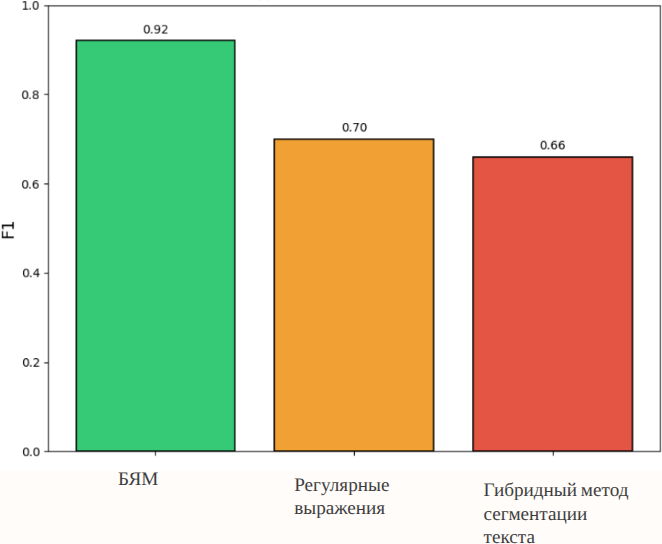
\includegraphics[width=0.9\linewidth]{images/vasexp.png}

  \caption{Эксперименты: визуализация и результаты} 
  \label{fig:vasexp}

\end{figure} 
\FloatBarrier

Эксперимент иллюстрирует, что для более точного извлечения библиографических областей требуется применение больших языковых моделей.

\section{Эксперимент на русскоязычном наборе данных}
Одной из ключевых проблем при проектировании систем интеллектуального парсинга библиографических данных является отсутствие в открытом доступе специализированных русскоязычных корпусов, размеченных в соответствии с национальными стандартами, в частности, ГОСТ. Большинство существующих наборов данных, таких как EXCITE или Grobid, ориентированы исключительно на англоязычную научно-техническую литературу и стандарты APA, MLA или Chicago. 

Для решения проблемы холодного старта и формирования репрезентативной выборки был рассмотрен массив из 7312 документов в формате  $\LaTeX$ (\texttt{*.tex}),  предоставленный специально для данной работы Математическим институтом им. В.А. Стеклова РАН. Массив документов содержит списки литературы к научным статьям, индексированным в базе данных Общероссийского математического портала Math-Net.Ru \cite{chebukov2013math}. Особенностью  данных является то, что для каждого пункта списка литературы представлены как оригинальная русская, так и переводная английская версии цитируемой публикации.

Процесс подготовки данных состоял из нескольких последовательных этапов:
\begin{enumerate}
    \item Нормализация кодировки текста: Исходные файлы поставлялись в устаревшей кодировке \texttt{CP866} (DOS Russian), использовавшейся в ранних дистрибутивах MiKTeX для совместимости с консольным выводом. Для корректной интеграции с современными токенизаторами БЯМ был разработан автоматизированный скрипт на языке Python, осуществивший пакетную транскодинговую конвертацию всего пула документов в международный стандарт \texttt{UTF-8}.
    \item Сегментация и экстракция макросов: Из структуры $\LaTeX$-документов с помощью регулярных выражений изолировалось содержимое окружения \texttt{\textbackslash begin\{thebibliography\}} \dots \texttt{\textbackslash end\{thebibliography\}}. Каждая запись, ограниченная макросами \texttt{\textbackslash Bibitem} или \texttt{\textbackslash RBibitem}, извлекалась как отдельный объект.
    \item Синтаксический разбор и конвертация: Внутренние теги издательской разметки (такие как \texttt{\textbackslash by} — авторы, \texttt{\textbackslash paper} — название статьи, \texttt{\textbackslash jour} — журнал, \texttt{\textbackslash yr} — год издания, \texttt{\textbackslash vol} — том, \texttt{\textbackslash issue} — номер, \texttt{\textbackslash pages} — страницы) парсились и агрегировались в структурированный формат \texttt{YAML}. 
    \item Генерация сырых строк по ГОСТ: На основе извлеченных атомарных полей программным путем формировалась монолитная текстовая строка («сырая» ссылка), имитирующая реальное текстовое представление пристатейного списка по ГОСТ.
\end{enumerate}

В результате выполнения описанного конвейера предобработки был сформирован итоговый профильный датасет, суммарно насчитывающий 19 430 уникальных библиографических записей, полностью готовых для проведения сравнительных экспериментов.

Целью данного этапа исследования являлось определение способности современной большой языковой модели общего назначения осуществлять синтаксический разбор без предварительного специализированного дообучения весов. 

Дизайн эксперимента строился по следующей схеме:
\begin{enumerate}
    \item Из сформированной базы данных \texttt{YAML} последовательно извлекалась сгенерированная «сырая» библиографическая строка.
    \item Строка передавалась в БЯМ в качестве входного параметра (\texttt{input}) в рамках жестко заданного системного контекста (System Prompt): \textit{«Ты — эксперт по библиографии. Извлеки данные в JSON: authors, paper, journal, year, volume, issue, pages. Если данных нет, пиши null. Отвечай ТОЛЬКО чистым JSON»}.
    \item Сгенерированный текстовый ответ модели валидировался на соответствие синтаксису JSON, десериализовался в Python-словарь и поэлементно сравнивался с эталонными полями разметки, полученными напрямую из исходных $\LaTeX$-макросов Math-Net.
\end{enumerate}

В качестве исследуемого вычислительного ядра была выбрана модель Llama-3-8B-Instruct, представленная в оптимизированном формате квантования Q4\_K\_M (4-битное квантование сбалансированного типа) в виде единого бинарного файла \texttt{.gguf}. Эксперимент разворачивался на CPU-сервере: 20 ядер, 78.5 Гб RAM под управлением инференс-движка \texttt{llama.cpp}. Использование квантованной модели 8B обусловлено необходимостью достижения приемлемой скорости генерации (в среднем 2.14 токена в секунду) в условиях отсутствия графических ускорителей (GPU).

Для математической оценки качества извлечения каждой из семи библиографических областей использовалась строгая метрика $F_1\text{-score}$, рассчитываемая на уровне отдельных токенов (Token-level) для нивелирования незначительных различий в знаках пунктуации, кавычках или служебных символах $\LaTeX$ (например, знаках неразрывного пробела \texttt{\~{}}):
\begin{equation}
Precision = \frac{|T_{true} \cap T_{pred}|}{|T_{pred}|}, \quad Recall = \frac{|T_{true} \cap T_{pred}|}{|T_{true}|}
\end{equation}
\begin{equation}
F_1 = 2 \cdot \frac{Precision \cdot Recall}{Precision + Recall}
\end{equation}
где $T_{true}$ — множество токенов в эталонном поле, а $T_{pred}$ — множество токенов в строке, извлеченной БЯМ. Общее качество модели оценивалось через интегральный показатель $Macro\ F_1$, представляющий собой среднее арифметическое оценок всех изолированных областей.

После проведения полного цикла инференса на тестовом подмножестве данных были зафиксированы показатели точности, представленные в таблице~\ref{tab:base_results}.

\begin{table}[h!]
\centering
\caption{Показатели точности извлечения данных базовой моделью Llama-3-8B-Instruct (Q4\_K\_M)}
\label{tab:base_results}
\begin{tabular}{|l|c|}
\hline
\textbf{Библиографическая область} & \textbf{Метрика Token-level $F_1$-score} \\ \hline
Авторы (\texttt{authors}) & 0,8766 \\ \hline
Название статьи/книги (\texttt{paper}) & 0,2700 \\ \hline
Журнал/Издательство (\texttt{journal}) & 0,8200 \\ \hline
Год издания (\texttt{year}) & 0,9951 \\ \hline
Том (\texttt{volume}) & 0,9613 \\ \hline
Номер выпуска (\texttt{issue}) & 0,9909 \\ \hline
Страницы (\texttt{pages}) & 0,9619 \\ \hline \hline
\textbf{Интегральный показатель Macro $F_1$} & \textbf{0,8397} \\ \hline
\end{tabular}
\end{table}


Анализ численных результатов позволяет сделать важные выводы о характере работы предобученной модели Llama-3 в задачах Zero-Shot парсинга русскоязычных академических текстов:
\begin{enumerate}
    \item Аномально низкое качество извлечения названий статей ($F_1 = 0,27$): Данный провал является центральной уязвимостью базовой модели. Его природа кроется в синтаксической специфике ГОСТ. В русскоязычной традиции название статьи графически никак не отделяется от авторов (идет сразу за ними через точку или пробел), но жестко отделяется от названия журнала двойным слэшем (\texttt{//}). Модель безошибочно определяла границу журнала, но стабильно «отрезала» значительную часть названия статьи, путая её с именами авторов, либо полностью игнорировала это поле, заполняя его значением \texttt{null}, если название содержало специфическую математическую терминологию.
    \item Высокая точность квазирегулярных сущностей: Поля «Год» ($0,9951$), «Номер» ($0,9909$) и «Страницы» ($0,9619$) распознаются моделью практически безошибочно. Это объясняется тем, что числовые паттерны, окруженные характерными маркерами (буквами «С.», «Т.», «№»), обладают сильной позиционной привязкой в механизме внутреннего внимания БЯМ, сформированной ещё на этапе предварительного обучения.
    \item Проблема языкового барьера: Поле «Авторы» ($0,8766$) продемонстрировало умеренное качество. Модель часто путалась в инициалах русских фамилий, склеенных через тильду или точку, иногда относя их к метаданным самой строки.
\end{enumerate}

Несмотря на относительно высокий интегральный показатель $Macro\ F_1 = 0,8397$, базовая архитектура Llama-3-8B-Instruct в режиме Zero-Shot непригодна для решения практических задач автоматизации библиографического контроля из-за критически низкой точности локализации названий публикаций ($F_1 = 0,27$). Модель демонстрирует глубокое непонимание специфики русскоязычных разделителей ГОСТ. Данный вывод полностью обосновывает необходимость перехода от инженерии промптов к технологиям глубокой адаптации весов модели под конкретную предметную область, что и легло в основу проведения следующего эксперимента по дообучению с использованием LoRA-адаптеров.

\section{Дообучение БЯМ с помощью LoRA-адаптера}
Для повышения качества извлечения библиографических областей из неструктурированных текстовых строк было принято решение о проведении экспериментов по контролируемому дообучению больших языковых моделей. Прямое полное дообучение всех параметров модели признано неэффективным ввиду высоких вычислительных затрат.

В связи с этим в качестве базового метода адаптации выбран алгоритм низкоранговой адаптации $LoRA$, а точнее его модификация, оптимизированная по объёму потребляемой памяти, -- $QLoRA$. $QLoRA$ внедряет небольшое число обучаемы весов, называемых адаптерами, в слои внимания замороженной базовой модели, предварительно квантованной в 4-битный форма нормализованного типа данных с плавающей запятов $NF4$.

Математическая суть модификации слоёв линейное проекции приведена в уравнении:
\begin{equation}
    W_{updated} = W_{base} + \Delta W = W_{base} + \frac{\alpha}{r} (A \cdot B)
\end{equation}
где $W_{base} \in \mathbb{R}^{d \times k}$ — замороженные веса базовой модели, $A \in \mathbb{R}^{d \times r}$ и $B \in \mathbb{R}^{r \times k}$ — матрицы низкого ранга, подлежащие обучению, $r$ — ранг адаптера ($r \ll \min(d,k)$), а $\alpha$ — коэффициент масштабирования слоев LoRA.

После чего был поставлен эксперимент на локальном CPU-сервере с 20 вычислительными ядрами процессора, 78,5 Гб оперативной памяти. В качестве среды выполнения использовалась библиотека $llama.cpp$ и её Python-обертка $llama-cpp-python$.

Однако в ходе отладки было выявлено критическое ограничение: бинарные компоненты и компилятор $llama-finetune$ на текущий момент развития экосистемы не поддерживают обратное распространение ошибки (backpropagation) через квантованные структуры тензоров (форматы типа $Q4\_K\_M$). Попытка запуска приводила к системному сбою ядра вычислений (`GGML\_ASSERT failed`). В связи с этим процесс обучения был перенесен в облачную инфраструктуру, оснащенную графическим ускорителем $NVIDIA\ Tesla\ T4$ с 16 Гб видеопамяти ($VRAM$).

Программный стек эксперимента составили:
\begin{itemize}
    \item Фреймворк высокоэффективного дообучения $Unsloth$;
    \item Библиотека управления обучением $Hugging\ Face\ TRL$ ($SFTTrainer$);
    \item Библиотека квантования $bitsandbytes$;
    \item Инструментарий визуализации $Unsloth\ Studio$.
\end{itemize}

Для проведения эксперимента из исходных файлов разметки $\LaTeX$ ($*\_utf8.tex$) подсистем библиографических списков журналов был сформирован массив данных, содержащий сырые строки и соответствующие им целевые JSON-объекты.

В ходе первой итерации автоматизированной разметки корпуса был зафиксирован систематический сдвиг левых границ извлекаемых сущностей, приведший к падению точности базовых моделей. Анализ ложноположительных срабатываний выявил ошибку избыточной предикации (\guillemotleft жадного квантификатора\guillemotright{}) в регулярных выражениях, отвечающих за первичный токенизированный парсинг. 

Применение оператора вида \texttt{.*} вместо его ленивой модификации \texttt{.*?} приводило к тому, что поисковый движок захватывал максимальную непрерывную последовательность символов. В контексте библиографии это вызывало поглощение конечных инициалов предыдущего автора началом названия статьи, либо слияние года издания с номерами страниц при совпадении синтаксических разделителей. Данный дефект разметки привел к искажению контекстных окон при обучении LoRA-адаптера, так как модель получала зашумленные векторы признаков $x_{ij}$.

Для стабилизации конвейера все жадные квантификаторы в регулярных масках были принудительно ограничены точками останова и переведены в ленивый режим работы. Повторная фильтрация корпуса исключила наложение смежных полей, что позволило повысить итоговое значение символьно-ориентированной метрики $F_1$ на этапе семантического структурирования. Сравнительный анализ структуры корректного и дефектного элементов датасета представлен в таблице~\ref{tab:dataset_error}.

\begin{table}[h!]
\centering
\caption{Анализ дефекта предобработки данных}
\label{tab:dataset_error}
\begin{tabular}{|l|p{5cm}|p{5cm}|}
\hline
\textbf{Поле JSON} & \textbf{Дефектный датасет (Итерация 1)} & \textbf{Корректный датасет (Итерация 2)} \\ \hline
\texttt{instruction} & Извлеки библиографические данные в JSON. & Извлеки библиографические данные в JSON. \\ \hline
\texttt{input} & Татаринов Я. В. Слабо неголономные системы // 1986. & Татаринов Я. В. Слабо неголономные системы // 1986. \\ \hline
\texttt{output} & Ты — эксперт по библиографии... & \{"authors": "Татаринов Я. В.", "paper": "Слабо неголономные системы", "year": "1986"\} \\ \hline
\end{tabular}
\end{table}

Именно этот скрытый дефект данных, обнаруженный в ходе пост-анализа, предопределил провал первой итерации обучения, так как модель была обучена замещать логику анализа простым циклическим копированием системного промпта.

Гиперпараметры LoRA-адаптера и процедуры обучения зафиксированы следующим образом: ранг адаптера $r = 16$, коэффициент $\alpha = 16$, целевые модули — все линейные слои ($q\_proj, k\_proj, v\_proj, o\_proj, gate\_proj, up\_proj, down\_proj$), скорость обучения $LR = 2\cdot 10^{-4}$ с линейным затуханием, оптимизатор — 8-битный $AdamW$. Базовая модель — $Llama-3-8B-Instruct$ ($bnb-4bit$). Всего было выполнено 100 шагов оптимизации с размером батча равным 2 и аккумулированием градиентов на 4 шага.

Несмотря на то, что графики функции потерь ($Loss$) в интерфейсе $Unsloth\ Studio$ демонстрировали идеальную сходимость, где замечено падение значения с 2,8 до 0,12, итоговое тестирование обученного LoRA-адаптера на контрольной выборке из 510 записей показало катастрофические результаты, усредненные по метрике $Macro\ F1$.

\begin{table}[h!]
\centering
\caption{Результаты тестирования дефектного LoRA-адаптера}
\label{tab:bad_results}
\begin{tabular}{|l|c|}
\hline
\textbf{Библиографическая область} & \textbf{Метрика Token-level F1-score} \\ \hline
Authors & 0,4039 \\ \hline
Paper & 0,3681 \\ \hline
Journal & 0,4014 \\ \hline
Year & 0,4039 \\ \hline
Volume & 0,4039 \\ \hline
Issue & 0,4039 \\ \hline
Pages & 0,4027 \\ \hline \hline
\textbf{Macro F1 Score} & \textbf{0,3983} \\ \hline
\textbf{Количество критических ошибок JSON} & \textbf{304 из 510} \\ \hline
\end{tabular}
\end{table}

Детальный анализ логов инференса (вывода) модели позволил локализовать природу аномалии. Модель не потеряла способность к генерации токенов, однако вместо формирования целевой структуры JSON, она циклически генерировала текст: \textit{«Ты — эксперт по библиографии. Извлеки данные в JSON. — — Извлеки библиографические данные в JSON...»}. 

Данное поведение обусловлено двумя факторами:
\begin{enumerate}
    \item Переобучение на мусорном паттерне (Data Poisoning): Из-за ошибки в скрипте конвертации $convert\_train2json.py$, модель выучила ложную статистическую взаимосвязь: на любую сырую строку отвечать текстом инструкции.
    \item Нарушение формата разметки токенов (Inference Prompt Mismatch): Несовпадение специальных токенов разметки начала и конца сообщений ($<|start\_header\_id|>$, $<|eot\_id|>$) во время обучения в GUI-студии и последующего скриптового тестирования привело к зацикливанию механизма внимания (Attention Loop). Модель интерпретировала управляющие токены как часть текстового ответа.
\end{enumerate}

Проведенный эксперимент наглядно иллюстрирует фундаментальный принцип инженерии данных: качество работы дообученной большой языковой модели прямо пропорционально качеству очистки и разметки входного датасета. Даже при идеальных показателях сходимости математической функции потерь на этапе обучения, дефекты структуры данных приводят к полной деградации целевой логики на этапе инференса. Данный опыт лег в основу разработки модифицированного, строго валидируемого конвейера подготовки данных, рассматриваемого в следующем разделе.